% !TEX root = ../main.tex
% !TEX program = XeLaTeX
% !TEX encoding = UTF-8 Unicode

\date{2018년 3월 7일}

\begin{frontmatter}
\title{레즈기어}
\author{양재영}
\address{서울대학교}
\begin{abstract}
Haspelmath, Martin. (1993). A Grammar of Lezgian. Berlin, Boston: De Gruyter Mouton.
\end{abstract}
\end{frontmatter}

%%%%%

\section*{발제 범위 분배}
\begin{table}[h]
\begin{center}
\def\arraystretch{1.5}
\begin{tabular}{>{\sffamily}ccccl}
\hline
	&\itshape 발제자	&\itshape 발제 범위
	&\itshape 페이지	&\itshape 내용\\
\hline
1	&양재영	&Ch. 1--4	&pp. 1--51			&서론, 화자, 분절음운단위, 음소배열론\\
2	&		&Ch. 5--7	&pp. 52--109		&(형태)음운적 교체, 강세, 명사 형태론\\
3	&		&Ch. 8--9	&pp. 110--162		&형용사 형태론, 동사 굴절\\
4	&		&Ch. 10--12	&pp. 163--227		&동사 파생, 대명사, 부사 \& 후치사\\
5	&		&Ch. 14--15	&pp. 228--293		&수사 \& 불변화사, 명사구 \& 형용사구, 동사 결합가\\
6	&		&Ch. 16--19	&pp. 294--353		&절 통사론, 계사절, 등위접속, 관계절\\
7	&		&Ch. 20--21	&pp. 354--400		&보문절, 부사절\\
8	&		&Ch. 22--24	&pp. 401--441		&공지시, 의문문, 비교\\
\hline
\end{tabular}
\end{center}
\label{default}
\end{table}

%%%%%

\section{서론}
\subsection{레즈기어와 그 계통적 분류}
\paragraph{} 레즈기어는 나흐다게스탄((북)동캅카스)어족 다게스탄어파 레즈기어군에 속하며, 캅카스 동부에 위치한 다게스탄 공화국 남부와 아제르바이잔 북부에서 약 40만명이 사용하는 언어이다. 1928년부터 라틴 문자로, 1938년부터는 키릴 문자로 표기되어 왔다. 이 문법서는 저지대 귀네 방언에 기반한 표준어를 다룬다. (북)동캅카스어족이라는 명칭은 카르트벨리(남캅카스)어족 및 압하스아디게((북)서캅카스)어족과 함께 하나의 어족을 이룬다는 오해를 피하기 위해 사용하지 않는다.
\subsection{레즈기어 문법 개관}
\subsubsection{음운론 및 형태음운론}
\begin{enumerate}
	\item 레즈기어의 모음 체계는 비대칭적이다. 자음은 54개로 풍부하다.
	\item 음절 구조는 CV(C(C))이며, 자음군은 어말이나 소수 단어의 형태소 경계에서 나타난다. 그러나 최근의 모음 탈락 현상으로 어두 자음군이 늘어나고 있다.
	\item 명사에서는 다양한 자음 교체가 일어난다.
	\item 단어의 두 번째 음절까지 전/후설 및 (비)원순 모음조화가 존재한다.
	\item 강세는 보통 두 번째 음절에 (단음절 어근은 첫 번째에도) 오며 아랍어 차용어는 세 번째 음절에 오기도 한다. 접미사는 강세 중립과 강세 유도의 두 가지가 있으며, 전자는 강세를 받지 않고 후자는 단음절 어근에만 붙어 강세를 받는다.
\end{enumerate}
\subsubsection{형태론}
\begin{enumerate}
	\item 레즈기어는 접미사가 지배적인 교착어이다. 명사, 형용사, 동사는 형태적 기준에 따라 쉽게 구별된다.
	\item 명사는 단/복수 및 격/위치에 따라 굴절한다. 위치격인 재격, 출격, 향격은 위치와 조합되어 나타난다. 절대격을 제외한 격은 많은 명사에 대해 고유한 접미사를 갖는 사격 어간을 동반한다.
	\item 동사는 시/상, 부정, 서법 몇 개와 다양한 비정형 굴절이 있다. 수/인칭 일치 형태는 없다.
	\item 파생 형태론은 빈약하며 차용된 파생 접사들도 존재한다.
\end{enumerate}
\subsubsection{통사론}
\begin{enumerate}
	\item 레즈기어의 어순은 핵어가 마지막에 오는 것이 지배적이다. 이는 명사구, 형용사구, 후치사구에서는 필수이고 절에서는 선호된다. 그러나 특히 구어에서는 SOV가 아닌 어순도 가능하다.
	\item 절에서의 격 표시는 능격 체계를 따른다. 일부 경험 동사에는 여격 주어가 나타난다.
	\item 레즈기어에는 일치가 전혀 없으며, 완전한 명사구 논항이 없으면 대명사가 보통 사용된다.
	\item 자동사를 타동사로 바꾸는 (사동) 파생접사 -ar-을 제외하면 문법적 관계를 바꾸는 규칙은 사실상 없다.
	\item 종속절은 보통 비정형이며 일반적으로 주절에 선행한다. 관계절은 분사를 사용하며 거의 모든 성분에 대해 관계화가 가능하다. 보문절에는 마스다르(동명사), 부정사, 분사 유형이 있다.
	\item wa ‘and’로 절을 등위접속할 수 있지만 부동사를 사용한 구문이 더 선호된다.
	\item 판정의문문은 접미사 -ni로 표시된다. 설명의문문에서는 접미사가 쓰이지 않고 의문대명사는 제자리에 있는다.
	\item 부등비교는 기준을 상출격으로 표시한다.
\end{enumerate}
\subsection{문법서에 대한 안내}
이 문법서는 분석적 관점(형태에서 기능으로)과 종합적 관점(기능에서 형태로)을 고루 사용했다. 전자는 주로 형태론, 후자는 주로 통사론 기술에 활용되었다.

\section{레즈기어와 그 화자}
\subsection{레즈기인}
레즈기인들은 캅카스 동부의 고산지 및 산맥과 카스피해 사이의 평야, 총 약 5천 제곱킬로미터의 영역(“레즈기스탄”)에서 살고 있으며, 구소련의 많은 주요 도시에 상당한 이주 인구가 있다. 1989년 기준 46만 6천 명의 레즈기인이 소련에 살고 있었으며, 언어 보존률이 약 90퍼센트였으므로 화자 수는 40만 명 이상일 것이다. 대부분의 레즈기인은 마을에 살며 농사(평야)와 목축(산지)으로 살아간다. 전통적으로 수니파 무슬림이며, 중동 세계 및 러시아와의 접촉은 레즈기어에 많은 차용어를 남겼다.
\subsubsection{인구 수치}
다게스탄의 레즈기인 마을에서는 언어 보존률이 100\%이지만 도시에서는 러시아어에 밀려 사라지는 추세였으며, 아제르바이잔의 레즈기인은 아제르바이잔인과의 동화를 강요당해 인구 통계에 오차가 있을 듯하다. (무엇보다 오래되었다. "30년이 되었습니다!")
\subsubsection{지리적 위치}
\omission
\subsubsection{레즈기사 개요}
\begin{itemize}
	\item 다게스탄은 7-8세기경 아랍인에게 정복되었다. 이로 인해 다게스탄 사람들은 이슬람으로 개종하게 되었다.
	\item 이후 여러 칸국들의 지배 하에 놓이다가, 19세기 초에 러시아 제국에 병합되기 시작했다. 일부 인구의 맹렬한 저항으로 1860년대까지도 완전히 러시아령이 되지 못했다. 패배한 레즈기인들은 추방당해 터키에 정착했다.
	\item 레즈기어의 표준 문어는 1920년대 후반에 도입되었고 학교 교육과 정규 출판에 사용되었다.
	\item 고르바초프의 개혁 이후 레즈기인들의 민족운동(Sadwal “Unity”)이 형성되었으며, 많은 레즈기인은 소련 해체 이후 다게스탄과 아제르바이잔으로 분리된 레즈기스탄에 대해 문제의식을 가지고 있다.
\end{itemize}
\subsubsection{레즈기라는 민족명}
\begin{itemize}
	\item 레즈기인들은 스스로를 lezgi라고 부르며, 이는 1920년대부터 지금과 같은 뜻으로 사용되어 왔다.
	\item 그 전에는 이 용어가 다게스탄의 모든 비튀르크 산악 민족에게 사용되었으며, 지금의 레즈기인과 레즈기어는 Küre 혹은 Küri라고 불렀다.\\(사실 이 이름은 외부인들에게 가장 접근성이 좋은 동부 평야의 방언명이다.)
	\item 여기에서는 다양한 영어명 중 lezgi와 유사하고 다른 언어학자들의 연구에서도 사용된 Lezgian이라는 철자를 사용한다.
\end{itemize}
\subsection{레즈기어의 방언}
다른 다게스탄어파 주요 언어들(다르과어와 아바르어 등)과 달리 레즈기어는 내적으로 방언 다양성이 적다. 표준어와의 차이는 비교적 사소하며 모든 방언이 상호 이해 가능하다.
\subsubsection{방언권 구분}
\begin{itemize}
	\item 레즈기어가 퀴레, 아흐체, 쿠바 방언권으로 삼분된다는 점은 대체로 합의된 사항이다.
	\item 퀴레 방언권은 다시 귀네, 꾸라, 자르끼 방언권으로 세분된다(Meljanova 1964).\\쿠바 방언권은 아제르바이자에 위치한다.
	\item 일부 저자는 특정 방언권에 속하지 않는 ‘혼합’ 방언들을 제시하기도 했다.
\end{itemize}
\subsubsection{방언별 특징}
\begin{itemize}
	\item 여러 방언(특히 아흐체)에는 추가적으로 후설 비원순 고모음 /ɨ/가 존재한다. /ɨ/와 /u/의 관계는 표준어의 /i/와 /y/의 관계와 유사하다.
	\item 또한 여러 방언에서, 특히 인두자음과 구개수 장애음 인접 환경에서 모음의 인두음화가 편재한다. 체페르 방언에는 전설 원순모음 /ø/가 존재한다.
	\item 여러 방언에 유/무성 인두 마찰음이 있으며 주로 아랍어 차용어에 나타나지만 종종 고유어에도 쓰인다.
	\item 양순음화된 후치경 장애음들이 존재하는 방언들도 있다.
	\item 아흐체 방언에서는 방출/유기 교체 대신 무기/유기 교체가 일어난다. 등등…
\end{itemize}
\subsection{레즈기어 및 그 표준어의 위상}
\begin{itemize}
	\item 19세기 중반까지 레즈기어는 구어와 구전 문학에서만 사용되었다. 종교, 관료, 사법, 명문에는 다게스탄 전 지역에서 아랍어가 사용되었다.
	\item 다게스탄과 아제르바이잔이 러시아 제국에 병합되었을 때 러시아어가 아랍어 대신 통치의 언어가 되었다. 또한 19세기 후반부터 여러 시인들이 아랍 문자로 시를 적기 시작했다.
	\item 페트르 카를로비치 우슬라르 남작이 레즈기어(Uslar 1896) 포함 캅카스 북부의 일곱 언어에 대한 훌륭한 기술을 남겼고, 러시아 키릴문자 기반의 알파벳을 고안했으나, 문어 보급에는 실패했다.
	\item 볼셰비키 혁명 후에는 라틴 문자, 퀴레 방언 (내에서도 귀네 방언) 기반의 표준어가 제정되었다. 해당 방언의 선정 이유는 화자가 가장 많고, 유명 시인들의 작품으로 잘 알려진 데다가, 우슬라르의 문법서가 퀴레 방언권의 한 방언을 기술했기 때문이다.
	\item 이후 키릴 문자 체계로 대체되었고, 고등 교육을 포함한 여러 수준에서 교육이 이루어졌다. 이러한 호의적 환경에도 불구하고 레즈기어 사용은 감소 추세이나, 시골 지역에서는 여전히 단일어 화자가 꽤 있으므로 사멸 위기 언어는 아니다.
\end{itemize}
\subsection{레즈기어에 대한 언어 접촉의 영향}
역사적으로 가장 중요한 접촉 언어들은 아제르바이잔어를 비롯한 튀르크어, 아랍어, 페르시아어, 러시아어이며 오늘날에는 아제르바이잔어와 러시아어만이 접촉을 유지하고 있다.
\begin{itemize}
	\item 전통적으로 무슬림인 민족의 언어인 만큼 레즈기어는 종교 용어뿐 아니라 많은 추상 및 고급 어휘(일부 일상 어휘)에서 아랍어 차용어가 상당한 역할을 한다. 접속사 wa도 아랍어 차용이다.
	\item 준-보문소로 쓰이는 불변화사 χi와 조건 불변화사 eger는 페르시아어 차용이다.
	\item 튀르크어의 영향은 다게스탄어파 내에서도 레즈기어에 특히 강하며, 모든 분야의 어휘에 차용이 일어났다.
	\item 러시아어를 구사하는 레즈기인들이 많아지면서 러시아어 차용 역시 흔해졌고 기존의 중동 언어 차용어를 대체한 러시아어가 표준어가 되기도 했다. 문어에서 러시아어 통사의 영향이 구어보다 더 클 것이며 이 문법서에서 종종 언급한다.
\end{itemize}


\section{분절적 음운 단위}
\subsection{정서법과 전자법}
레즈기어 정서법에서는 러시아어에 쓰이는 모든 키릴 문자에 더해 I와 12개의 이합자가 사용된다. <I>는 이합자에만 쓰이며 파열음의 방출성을 나타낸다.
\begin{figure}[h]
\begin{center}
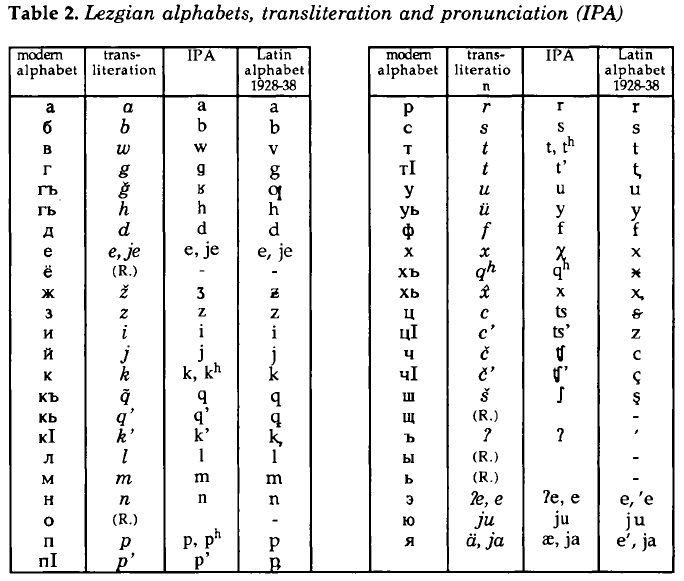
\includegraphics{Lezgian/src/lezalpha}
\end{center}
\label{레즈기어 알파벳}
\end{figure}
\subsubsection{표2에 대한 첨언}
\omission
\subsubsection{음소적 철자법에서의 예외 사항}
레즈기어 정서법은 대체로 음소적이지만 다음과 같은 사항에서 예외가 있다.
\begin{enumerate}
	\item 음소의 양순음화는 <в>로 표시된다. 그러나 단음소 /Cʷ/와 2음소 연쇄 /Cw/의 대립이 한 형태소 안에서는 드물기 때문에 심각한 문제는 아니다.
	\item 다음 음소들의 유무기 대립은 표기에 반영되지 않는다. 단 두 쌍만이 표기에 유/무기 대립을 반영한다.
	\item 최근에 시작된 어중 모음 탈락은 매우 비일관적으로 표기에 반영되어 있다.
\end{enumerate}
이외에는 상당히 음소적이므로 이 문법서에서는 로마자로 전자된 정서법을 활용할 것이며, 필요한 경우 IPA를 병기한다.
\subsection{모음}
\subsubsection{모음 목록}
레즈기어의 모음은 다음과 같다.
\begin{tabular}{l|cc|cc}
\hline
		&전 		&설		&후 	&설\\
		&비원순		&원순	&비원순	&원순\\
고모음	&i 			&y <ü>	&		&u\\
중모음	&e  		&		&		&\\
저모음	&æ(ː) <ä>	&		&a(ː)	&\\
\end{tabular}
\subsubsection{변이음}
\begin{enumerate}
	\item 표준어에서 모음 /æ/는 어간에서 비교적 드물며 단 하나의 접미사에서만 나타난다. 많은 방언에서는 이 모음이 더 자주 나타나며 다소 인두음화된다. 이 모음이 나타나는 어근 중 대부분은 인두음이 들어간 아랍어 기원 차용어이다. 표준어에서는 어두에 나타나지 않는데 이는 표기법에서 해당 글자가 /ja/를 나타내기 때문일 수도 있다. 귀네 방언에서 이 모음으로 시작하는 모든 단어는 /e/로 시작한다. 그러나 표준어에서도 몇몇 단어와 -äǧun으로 끝나는 동사군에서 이 모음이 나타난다.
	\item 두 종류의 장모음은 다소 애매한 지위를 가지고 있다. jaǧun 및 -äǧun 동사군에 자음으로 시작하는 접미사가 붙어 /ʁ/이 탈락하는 경우 보상적 장음화에 의해 나타난다. 또한 접미사의 -aj 및 -äj 역시 종종 /aː/와 /æː/로 각각 발음되나 필수는 아니다.
	\item /a/는 화자들이 다르다고 느끼는 두 가지 주 변이음(중모음 [ʌ]와 저모음 [a])이 있다. 후자는 폐음절의 구개수음이나 /r/ 앞에서 나타나며 전자는 나머지 경우에 나타난다. 그러나 [a]의 실현 환경이 확정된 것은 아니며, 양순음화된 자음 뒤에서는 종종 [ɔ]로 원순화된다.
	\item /e/는 강세 음절에서 [ɛ], 강세 앞 음절에서 [e]나 [i]로 발음된다. 이로 인해 철자상의 변이형이 존재할 수 있다. 양순음화된 자음 옆에서는 [ø]나 [œ]로 원순음화되기도 한다.
\end{enumerate}
\subsection{자음}
\subsubsection{자음 목록}
레즈기어의 자음은 다음과 같다.\\
\resizebox{19cm}{!}{
\begin{tabular}{cc|lllllllllll}
\hline
		&		&순음	&치음 	&			&	&치찰음&							&연구개음&			&구개수음&\\
		&		&		&		&			&치 		&음			&후치경음	&		&			&		&\\
	&(순음화)		&		&X 		&O 			&X			&O			&			&X  	&O			&X		&O\\
\hline
폐쇄음 	&유성 	&b		&d		&			&			&			&			&g		&gʷ			&		&\\
		&유기 	&pʰ <p>	&tʰ <t>	&tʰʷ <tw>	&ʦʰ <c>		&ʦʰʷ <cw>	&ʧʰ <č>		&kʰ <k>	&kʰʷ <kw>	&qʰ <q>	&qʰʷ <qw>\\
		&무기 	&p		&t		&tʷ			&ʦ <c>		&ʦʷ <cw>	&ʧ <č>		&k		&kʷ			&q		&qʷ\\
		&방출 	&pʼ		&tʼ		&tʼʷ		&ʦʼ <cʼ>	&ʦʼʷ <cʼw>	&ʧʼ	<čʼ>	&kʼ		&kʼʷ		&qʼ		&qʼʷ\\
\hline
마찰음	&유성 	&		&		&			&z			&zʷʼ		&ʒ <ž>		&		&			&ʁ <ǧ>	&ʁʷ <ǧw>\\
		&무성	&f		&		&			&s			&sʷ			&ʃ <š>		&x <x̂>	&			&χ <x>	&χʷ <xw>\\
\hline
\end{tabular}}
\begin{tabular}{l|cc}
\hline
비음	&m	&n\\
\hline
유음	&l	&r\\
\hline
활음	&j	&w\\
\hline
후음	&h	&ʔ\\
\hline
\end{tabular}\\
이외에도 방언마다 추가적인 음소가 존재한다. 양순음화된 치조 파찰음은 체계의 일부이나 극히 드물다. 어중 모음 탈락 현상으로 구개음화된 장애음 계열이 생겨났으나 이는 최근의 변화이므로 연구가 더 필요하다.
\subsubsection{변이음}
\begin{enumerate}
	\item 양순음화된 자음들은 후행 모음이 원순모음이면 그 영향으로 양순음성을 잃는다. 많은 방언에서 양순음화는 완전히 사라졌다.
	\item /l/는 후설모음 뒤 종성 위치에서 연구개음화되고 초성이나 전설모음 뒤에서는 “맑다”.
	\item /w/는 종종 양순/순치 마찰음으로 발음된다.
	\item /Vn/ 연쇄에서 모음이 후행하지 않으면 /n/은 선행 모음의 비음화를 수반하며 탈락하기도 한다.
	\item /nC/ 연쇄에서 C가 연구개/구개수 장애음이면 (탈락하지 않은) /n/은 C와 같은 조음 위치로 동화된다. 양순음 앞에서는 /m/과 /n/이 구별된다. /r/은 무성 장애음 사이에서 무성음화된다.
\end{enumerate}

\section{음소배열론}
\subsection{어중 모음 탈락}
\subsubsection{강세 앞 고모음 탈락}
최근에 일어나고 있는 현상으로서, 강세 앞에 오는 고모음이 무성 장애음 뒤에서 탈락한다. 이러한 어중 모음 탈락은 표준 정서법에는 대체로 반영되지 않는다. 이 문법서에서는 이 현상을 종종 pre-syncope라고 부를 것이다. 탈락한 모음이 철자에 반영되는 것은 선행 장애음에 탈락한 모음과 관련 있는 자질이 남기 때문일 수 있다. 예컨대 kifer '땋은 머리' /kʰʲfer/, tupʼal '반지' /tʰʷpʼal/, küče '거리' /kʰᶣʧe/. 그러나 이는 그렇게 규칙적이지 않아 보인다. 또한 단음절 단어와 같이 탈락이 일어나지 않는 단어와의 유추 작용으로 모음이 더 잘 보존되기도 한다. 마찰음 사이에서는 일반적으로 모음이 탈락하지 않으며, 장애음과 공명음 사이에서는 탈락하지 않을 수도 있다.
\subsubsection{강세 뒤 모음 탈락}
강세 뒤의 비어말 음절의 모음은 뒤에 자음이 하나만 오면 탈락하는 경향이 있다. 그러나 이는 강세 앞 모음 탈락보다 더 조건을 파악하기 어렵다. 고모음이 탈락하기 쉬우나 /a/가 탈락하는 경우도 있다.
\begin{enumerate}
	\item 미완료 부동사 + awa = 미완료, 부정과거 부동사 + awa = 완료 (+ ama = 계속). 이 경우 강세 뒤에 오는 /a/가 자음 뒤에서는 탈락하고 모음 뒤에서는 보존되며, 어중 모음이 둘이면 첫 번째 모음이 탈락한다. 그러나 어떤 방언에서는 /a/가 대신 탈락한다.
	\item 복수형 -ar의 /a/와 복수 명사화 -bur의 /u/ 역시 이로 인해 탈락할 수 있다.
	\item 출격의 비강세 어간 모음은 탈라락하기도 하나 표준 철자법은 아니다.
	\item 비강세 -ar로 끝나는 2음절 동사는 모음으로 시작하는 접미사가 붙으면 /a/가 탈락한다.
\end{enumerate}
\subsection{음절 구조}
\subsubsection{어중 모음 탈락 이전의 CV 구조}
레즈기어 단어의 음절 구조는 최근의 모음 탈락으로 크게 변했다. 여기서는 먼저 그 이전 시기 레즈기어의 음절 구조를 다루고, 이후 현재의 상태를 기술한다. 당시의 레즈기어는 CV(C(C)) 구조만을 허용했다. 어두에는 초성이 없을 수 있으며, 음절말 자음군은 어근 끝에서만 가능하다. 따라서 한 형태소 안에서는 2자음 연쇄만이 가능하다. 3자음 연쇄는 -CC로 끝나는 어근에 자음으로 시작하는 접미사가 붙어 나타난다. 자음군으로 시작하는 접미사는 없으므로 4자음 이상 연쇄는 레즈기어에서 나타날 수 없다. 일반적으로 모든 비어두 음절은 하나의 자음으로 시작하나, 일부 아랍어 차용어는 (성문 파열음이 들어가기도 하는) 모음으로 시작하는 어중 음절이 들어있다.
\subsubsection{어중 모음 탈락 이전의 형태소 내 자음군}
여기서는 형태소 내에서 가능한 자음군을 기술하며, 사용하는 약자는 다음과 같다. T = 장애음, L = 유음, N = 비음, W = 활음, R = 공명음, H = 후음. 이는 고유어와 차용어에서 약간 다르다.
다양하고 괴상한 자음군이 가능하지만 전체 목록을 소개하는 것은 소모적이므로 생략한다.
\subsubsection{어중 모음 탈락 이후의 음절 구조}
강세 앞 고모음 탈락으로 인해 어두에서 CC- 혹은 CCC- 연쇄까지도 흔해졌다. 예컨대 ptul '증손주', štkana '쓸었다'. 2음절에 강세가 오는 경우가 많았으므로 사실상 1음절에서만 모음 탈락이 일어났고 따라서 이러한 자음군은 어두에서만 가능하다. 강세 앞 모음 탈락의 조건 때문에 CC-는 무성 장애음 두 개 혹은 무성 장애음과 공명음으로 구성되며, CCC- 연쇄는 무성 장애음 세 개 혹은 무성 장애음 두 개와 그 사이의 /r/로 이루어져 있다. 
\subsection{자음 출현 제약}
\begin{enumerate}
	\item 무성 폐쇄음/마찰음 앞의 무성 폐쇄음은 항상 유기음이다. 이는 모음 탈락으로 인해 인접하게 된 경우에도 동일하다.
	\item 무성 폐쇄음/마찰음 뒤의 무성 폐쇄음은 항상 무기음이다. 이는 모음 탈락으로 인해 인접하게 된 경우도 동일하며, 위의 규칙이 우선 적용된다.
	\item 강세 모음 뒤에서 무성 폐쇄음은 위의 규칙이 적용되지 않는 한 항상 유기음이다. 이는 강세 모음 직후에 오지 않더라도 적용된다. 그러나 무성 마찰음 바로 뒤에 오는 경우 위의 규칙이 우선 적용된다.
	\item 방출 폐쇄음으로 시작하는 단어의 두 번째 음절은 무기무성 폐쇄음으로 시작할 수 없고 항상 유기음화가 일어난다.
	\item 두 음절 이상의 단어에서 강세 음절의 첫 번째 자음이 무기무성 폐쇄음이면 어두 무성 폐쇄음도 항상 무기음이다.
\end{enumerate}
\subsection{모음조화}
레즈기어 고유어 단어에서는 강세 음절과 그 앞의 음절들에 한해 전/후설과 (비)원순 모음조화가 존재한다. 고유어는 강세가 제2음절을 넘어가지 않으므로 적용되는 모음은 두 개를 넘지 않는다.
\subsubsection{전/후설 모음조화}
전/후설 모음조화는 전설모음 /e, i, y, æ/와 후설모음 /a, u/ 간의 대립을 보인다. 예외적으로 /a-i/ 및 /i-a/ 연쇄는 허용된다. 페르시아어, 아랍어, 러시아어에서 온 동화된 차용어가 많아 이 조화가 깨지는 어근도 있다.
\subsubsection{원순성 모음조화}
원순성 모음조화는 원순모음 /u, y/와 비원순모음 /i/ 간에 대립을 보인다. 저/중모음은 이 조화에서는 중립이다. 전/후설 모음조화에 의해, 이 제약으로 금지되는 조합은 */i-y/와 */y-i/ 뿐이다. 레즈기어가 /y/가 들어간 단어를 차용한 튀르크어에도 이러한 조화가 존재하므로 차용어에서도 예외 없이 적용된다.
\subsection{순음 장애음과 모음의 조화}
순음화된 장애음에 인접한 원순성 대립에 중립적이지 않은 모음은 원순모음이 된다. 따라서 */iCʷ/와 */Cʷi/는 금지되지만 wil '눈[眼]'이나 qʼiliw '가까운'은 가능하다. 이 제약으로 인해 비강세 모음 상승은 순음화된 장애음이 들어가는 어근에서 /e-y/ 교체를 일으킨다. 레즈기어 고유어에서 /y/는 이 규칙이나 위의 규칙으로 인해 나타나는 경우가 대부분이다. 따라서 고유어에서는 해당 모음이 거의 변별적이지 않으나, 튀르크계 차용어와 여러 음성 상징어로 인해 오늘날의 레즈기어에서는 변별적인 음소이다.
\subsection{장애음 순음화의 중화}
원순모음 앞에서 자음은 자동적으로 음성적으로 순음화된다. 17개의 순음화 계열 장애음은 이 환경에서 대립이 중화되므로 철자에 순음화가 반영되지 않는다. 형태음운상 존재하는 순음화는 괄호 안에 나타낸다. 마지막 음절의 모음이 원순인 경우에도 동일한 중화가 일어나며, 비원순이어도 철자에 순음화가 보존되지만 항상 그렇게 발음되지는 않는다.